\section{Theorie}
Ein Hohlleiter ist ein Metallrohr, indem Energie transportiert werden kann.
In diesem Versuch wird ein rechteckiger Hohlleiter verwendet, es gibt aber
auch eliptische oder runde Rohlleiter.

In einem Hohlleiter können elektromagnetische Schwingungen in verschiedenen Moden weitergeleitet werden. Jeder Modus besitzt eine Cut-Off-Frequenz, welche durch die Abmessung des Hohlleiters bestimmt wird. Unter dieser Freuquenz kann keine Energie weitergeleitet werden.
Es wird zwischen zwei Moden unterschieden: der "transversal elektrischen" (TE-Modus) und der "transversal magnetischen" (TM-Modus) Mode. Hierbei steht das jeweilige Feld überall senkrecht auf der Ausbreitungsrichtung bzw. der Hohlleiterachse. Ein Spezialfall ist die Überlagerung beider Moden: Bei dem TEM-Modus steht sowohl das magnetische als auch das elektrische Feld senkrecht zur Ausbreitungsrichtung (wie bei einer freien elektromagnetischen Welle oder einem Koaxialleiter). Die Indizes an dem Modus beschreiben die Anzahl der Halbwellen des Feldes in die zwei Hauptrichtungen. Als Beispuel ist in Abbildung \ref{abb:1} der $\text{TE}_{\symup{1,0}}$-Modus in einem rechteckigen Hohlleiter zu sehen.

\begin{figure}
  \centering
  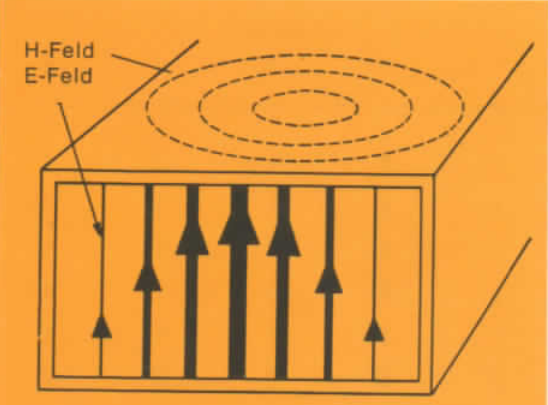
\includegraphics[scale=0.25]{Mode_1_0.png}
  \caption{$\text{TE}_{\symup{1,0}}$-Modus in einem rechteckigen Hohlleiter.}
  \label{abb:1}
\end{figure}

In Abbildung \ref{abb:2} ist das Blockschaltbild eines Klystron zu sehen.
Ein Klystron ist eine Mikrowellenröhre, bei der aus einem kontinuierlichen Elektronenstrahl mittels Geschwindigkeitsmodulation Mikrowellenenergie gewonnen wird. Hierbei werden Elektronen aus der Kathode emittiert und in Richtung der Gitter beschleunigt. Der Reflektor hat gegenüber der Kathode ein negatives Potential, sodass die Elektronen reflektiert werden. Somit durchlaufen die Elektronen erneut das Resonatorgitter. Fängt das Klystron an zu schwingen, werden die Elektronen entweder beschleunigt oder verzögert, abhängig vom Spannungsverlauf. Durch die verschiedenen Geschiwindigkeiten und somit verschiedenen Laufzeiten, entstehen durch die rückkehrenden Elektronen Bündel. Bei einer Abbremsung der Elektronen im Bündel wird Energie an den Resonator abgegeben und das Klystron fängt an zu schwingen. Die größte Schwingung tritt bei einer Verweilzeit im Resonator von $n+3/4$ Perioden der Resonatorfrequenz auf ($n\in \mathbb{N}_0$). Bei Beschleunigung der Elektronen im Bündel wird dem Resonator Energie entzogen und es kann somit keine Schwingung auftreten.

\begin{figure}
  \centering
  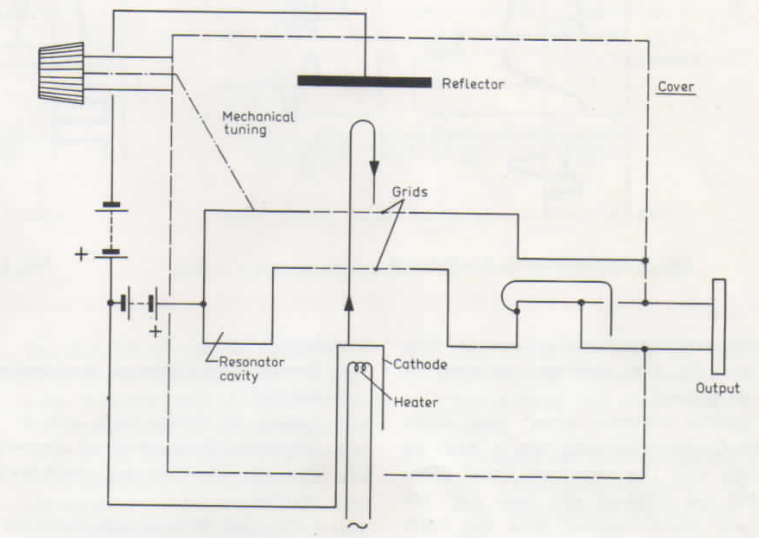
\includegraphics[scale=0.4]{Blockschaltbild.png}
  \caption{Blockschaltbild des Klystron.}
  \label{abb:2}
\end{figure}
